\documentclass[paper=a4, fontsize=11pt]{scrartcl} 

\usepackage[T1]{fontenc} 
\usepackage[english]{babel}
\usepackage{amsmath,amsfonts,amsthm}
\usepackage{lipsum}
\usepackage{graphicx}
\usepackage{float}
  \floatplacement{figure}{H}
  \floatplacement{table}{H}
  
\usepackage{sectsty} 
\allsectionsfont{\centering \normalfont\scshape} 

\usepackage{fancyhdr} % Custom headers and footers
\pagestyle{fancyplain} % Makes all pages in the document conform to the custom headers and footers
\fancyhead{} % No page header - if you want one, create it in the same way as the footers below
\fancyfoot[L]{} % Empty left footer
\fancyfoot[C]{} % Empty center footer
\fancyfoot[R]{\thepage} % Page numbering for right footer
\renewcommand{\headrulewidth}{0pt} % Remove header underlines
\renewcommand{\footrulewidth}{0pt} % Remove footer underlines
\setlength{\headheight}{13.6pt} % Customize the height of the header

\numberwithin{equation}{section} % Number equations within sections (i.e. 1.1, 1.2, 2.1, 2.2 instead of 1, 2, 3, 4)
\numberwithin{figure}{section} % Number figures within sections (i.e. 1.1, 1.2, 2.1, 2.2 instead of 1, 2, 3, 4)
\numberwithin{table}{section} % Number tables within sections (i.e. 1.1, 1.2, 2.1, 2.2 instead of 1, 2, 3, 4)

\setlength\parindent{0pt} % Removes all indentation from paragraphs - comment this line for an assignment with lots of text

\usepackage[labelformat=empty]{caption}
\usepackage{color}
\usepackage{listings}
\lstset{ %
language=bash,                % choose the language of the code
basicstyle=\footnotesize,       % the size of the fonts that are used for the code
numbers=left,                   % where to put the line-numbers
numberstyle=\footnotesize,      % the size of the fonts that are used for the line-numbers
stepnumber=1,                   % the step between two line-numbers. If it is 1 each line will be numbered
numbersep=5pt,                  % how far the line-numbers are from the code
backgroundcolor=\color{white},  % choose the background color. You must add \usepackage{color}
showspaces=false,               % show spaces adding particular underscores
showstringspaces=false,         % underline spaces within strings
showtabs=false,                 % show tabs within strings adding particular underscores
frame=single,           % adds a frame around the code
tabsize=2,          % sets default tabsize to 2 spaces
captionpos=b,           % sets the caption-position to bottom
breaklines=true,        % sets automatic line breaking
breakatwhitespace=false,    % sets if automatic breaks should only happen at whitespace
escapeinside={\%*}{*)}          % if you want to add a comment within your code
}

%----------------------------------------------------------------------------------------
%	TITLE SECTION
%----------------------------------------------------------------------------------------

\newcommand{\horrule}[1]{\rule{\linewidth}{#1}} % Create horizontal rule command with 1 argument of height

\title{	
\normalfont \normalsize 
\textsc{Computational Science - ITB} \\ [25pt] % Your university, school and/or department name(s)
\horrule{0.5pt} \\[0.4cm] % Thin top horizontal rule
%\huge  Summary - Euler Method\\ % The assignment title
%\horrule{2pt} \\[0.5cm] % Thick bottom horizontal rule
}

\author{\small{Ridlo W. Wibowo || 20912009}} % Your name

\date{\normalsize\today} % Today's date or a custom date

\begin{document}

\maketitle % Print the title

\large \textbf{Problem.}
Buatlah program untuk solusi Parabolic Partial Differential Equations (PDE),\\
- \textit{Forward Difference Method} (FTCS)\\ 
- \textit{Backward Difference Method} (BTCS)\\
- \textit{Crank-Nicolson Method} (C-N)\\
Lalu tentukan solusi untuk PDE:\\
\begin{equation}
\frac{\partial u}{\partial t} = \frac{\partial ^{2}u}{\partial x^{2}}
\end{equation}
untuk $0 < x < \pi$ dan $t > 0$ dengan,
\begin{itemize}
\item syarat batas:\\
$u(0, t) = u(\pi, t) = 0.0$ untuk $t > 0$\\
\item syarat awal:\\
$u(x,0) = \sin(x)$ untuk  $0 \leq x \leq \pi$\\ 
\end{itemize}
Gunakan $h=\frac{\pi}{10}$ dan $k=0.05$ dan bandingkan hasilnya untuk $t = 0.5$.\\
(solusi eksak $u(x, t) = e^{-t}\sin{x}$)\\


\newpage
\large \textbf{Result.}
Dari penurunan dan algoritma yang diberikan di buku \textit{Numerical Analysis} oleh Richard L.Burden dan J. Douglas Faires, lalu dapat diterapkan untuk membuat program penyelesaian masalah PDE. Program yang telah dibuat terlampir di akhir (\textit{ftcs.cpp}, \textit{btcs.cpp}, \textit{CN.cpp}).\\

\begin{itemize}
\item Tabel FTCS
\begin{table}[ht]
\begin{tabular}{c c c c}
\hline
$x_{i}$ & $u_{(x_{i}, 0.5)}$ & $w_{(x_{i}, 0.5)}$ & $\vert u - w \vert _{(x_{i}, 0.5)}$  \\ [0.5ex]
\hline 
0 & 0 & 0 & 0\\
0.314159 & 0.187428 & 0.18582 & 0.001608 \\
0.628319 & 0.35651 & 0.35345 & 0.00306 \\
0.942478 & 0.490694 & 0.486482 & 0.004212\\
1.25664 & 0.576845 & 0.571894 & 0.004951\\
1.5708 & 0.606531 & 0.601325 & 0.005206 \\
1.88496 & 0.576845 & 0.571894 & 0.004951 \\
2.19911 & 0.490694 & 0.486482 & 0.004212\\
2.51327 & 0.35651 & 0.35345 & 0.00306\\
2.82743 & 0.187428 & 0.18582 & 0.001608\\
3.14159 & 0 & 0 & 0\\ [1ex]
\hline 
\end{tabular}
\end{table}

\item Tabel BTCS
\begin{table}[ht]
\begin{tabular}{c c c c}
\hline
$x_{i}$ & $u_{(x_{i}, 0.5)}$ & $w_{(x_{i}, 0.5)}$ & $\vert u - w \vert _{(x_{i}, 0.5)}$  \\ [0.5ex]
\hline 
0	& 0	& 0	& 0 \\
0.314159	 & 0.187428 & 0.190452 &	 0.003024\\
0.628319 & 0.35651	& 0.362261 &	 0.005751\\
0.942478	 & 0.490694	& 0.498609 &	 0.007915\\
1.25664	& 0.576845 & 	0.58615 &	0.009305\\
1.5708	& 0.606531	 & 0.616315 &	0.009784\\
1.88496 &	0.576845 &	0.58615 &	0.009305\\
2.19911 &	0.490694	 & 0.498609 &	0.007915\\
2.51327 &	0.35651	& 0.362261 & 	0.005751\\
2.82743 & 0.187428 & 	0.190452	 & 0.003024\\
3.14159 &	0	& 0 &	0 \\[1ex]
\hline 
\end{tabular}
\end{table}

\newpage
\item Tabel Crank-Nicolson
\begin{table}[ht]
\begin{tabular}{c c c c}
\hline
$x_{i}$ & $u_{(x_{i}, 0.5)}$ & $w_{(x_{i}, 0.5)}$ & $\vert u - w \vert _{(x_{i}, 0.5)}$  \\ [0.5ex]
\hline 
0	& 0	& 0	& 0\\
0.314159	 & 0.187428	& 0.188179	& 0.000751\\
0.628319 &	0.35651	& 0.357938	& 0.001428\\
0.942478	 & 0.490694	& 0.492659	& 0.001965\\
1.25664	& 0.576845	& 0.579155	& 0.00231\\
1.5708	& 0.606531	& 0.60896	& 0.002429\\
1.88496	& 0.576845	& 0.579155	& 0.00231\\
2.19911	& 0.490694	& 0.492659	& 0.001965\\
2.51327	& 0.35651	& 0.357938	& 0.001428\\
2.82743	& 0.187428	& 0.188179	& 0.000751\\
3.14159	& 0	& 0	& 0 \\ [1ex]
\hline 
\end{tabular}
\end{table}
\end{itemize}

Perbandingan Error
\begin{table}[ht]
\begin{tabular}{c c c c}
\hline
$x_{i}$ & 	ftcs	 & btcs	& CN \\ [0.5ex]
\hline 
0.314159 & 	0.001608 & 	0.003024	 & 0.000751\\
0.628319	 & 0.00306	& 0.005751	& 0.001428\\
0.942478	 & 0.004212	& 0.007915	& 0.001965\\
1.25664	& 0.004951	& 0.009305	& 0.00231\\
1.5708	& 0.005206	& 0.009784	& 0.002429\\
1.88496	& 0.004951	& 0.009305	& 0.00231\\
2.19911	& 0.004212	& 0.007915	& 0.001965\\
2.51327	& 0.00306	& 0.005751	& 0.001428\\
2.82743	& 0.001608	& 0.003024	& 0.000751\\ [0.5ex]
\hline
max:	& 0.005206	& 0.009784	& 0.002429\\ [0.5ex]
\hline 
\end{tabular}
\end{table}

Dengan nilai $k$ dan $h$ sesuai persoalan untuk $t = 0.5$ ternyata ketiga metode konvergen, dan yang paling baik adalah \textit{Crank-Nicolson}. Metode FTCS dengan nilai $\lambda = 0.506606 \hspace{0.25cm} (> 0.5)$, ternyata masih konvergen.

\newpage
Kondisi Akhir ($t = 0.5$)
\begin{figure}
	\centering
	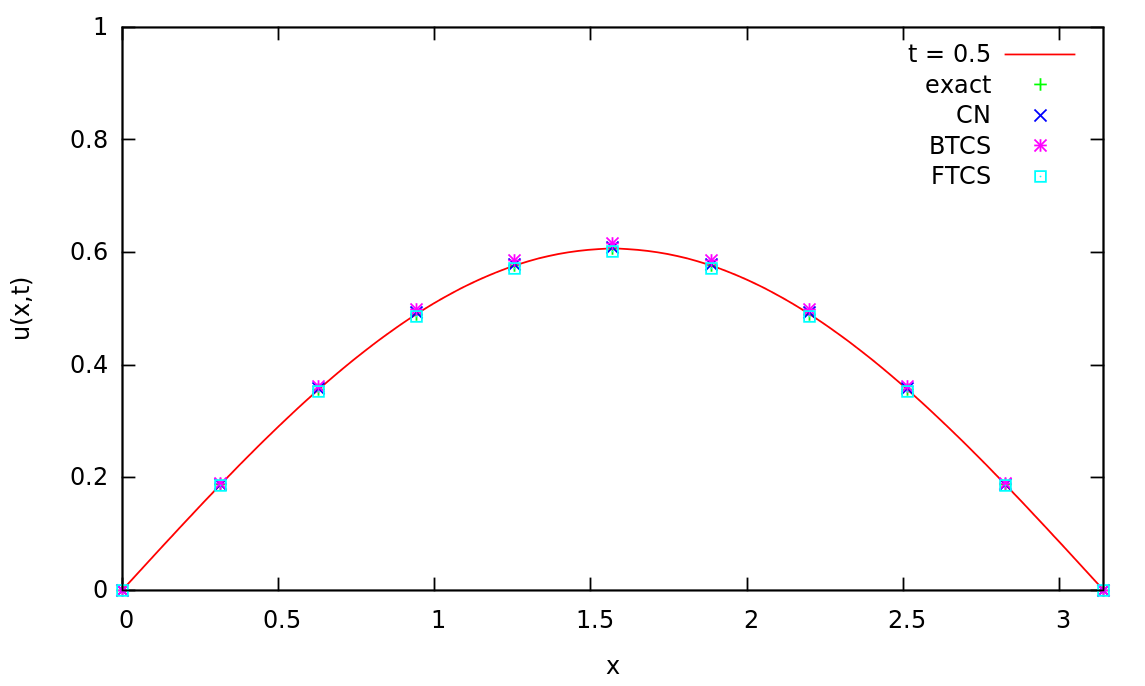
\includegraphics[width=0.8\textwidth]
		{plot.png}
	\caption{Plot hasil akhir ($t = 0.5$).}
\end{figure}

\begin{figure}
	\centering
	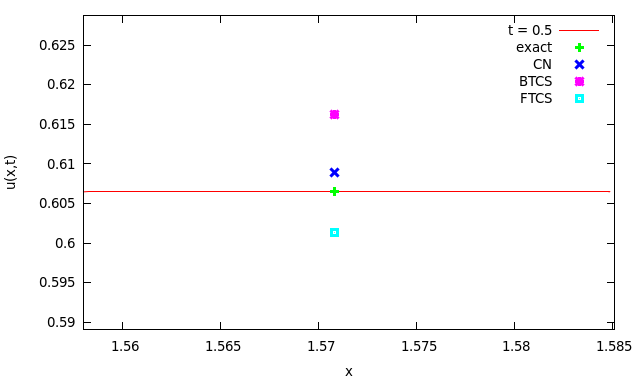
\includegraphics[width=0.8\textwidth]
		{zoom.png}
	\caption{Diperbesar disekitar $x = \frac{\pi}{2}$ ($t = 0.5$).}
\end{figure}

\newpage
\large \textbf{LAMPIRAN} \\
\large \textit{ftcs.cpp}
\lstset{frameround=fttt}
\begin{lstlisting}
/************************************************/
/* ftcs.cpp (forward time central space)        */
/* forward difference method - parabolic PDE    */
/* Copyleft (c) 2012. Ridlo W. Wibowo           */
/************************************************/
#include <iostream>
#include <math.h>
#include <stdlib.h>
#include <stdio.h>
#include <fstream>
#define _USE_MATH_DEFINES
using namespace std;

int main(){
    cout << "### Parabolic PDE - Forward Difference Method ###\n";
    cout << "--- Equation : d(u)/dt = d^2(u)/dx^2 with u(x,t) ---\n";
    double xi = 0.0, xf=M_PI; // L=1.0 -> rentang x
    double ti = 0.0, tf=0.5; // time
    int nt = 10; // jumlah pemenggalan di t
    int nx = 10; // jumlah pemenggalan di x

    double k = (tf-ti)/nt;
    double h = (xf-xi)/nx;
    
    double alpha = 1.;
    double lam = alpha*alpha*k/(h*h);
    cout << "alpha         = " << alpha << endl;
    cout << "step in x (h) = " << h << endl;
    cout << "step in t (k) = " << k << endl;
    cout << "lambda        = " << lam << endl;

    double wi[100];
    double wf[100];
    double x[100];

    // syarat batas
    wi[0] = 0.0;
    wi[nx] = 0.0;
    
    // syarat awal
    x[0] = xi;
    x[nx] = xf;
    for (int i=1; i<nx; i++){
        x[i] = x[i-1] + h;
        wi[i] = sin(x[i]);}
    
    // bentuk output filenya aneh, karena untuk 
    // mempermudah ketika membuat animasi memakai gnuplot
    ofstream out("ftcs-out.txt");
    // print kondisi awal
    for (int i=0; i<=nx; i++){
        out << x[i] << " " << wi[i] << "\n";}
    
    // kerjo dimulai.. ayo
    for (int j=1; j<=nt; j++){
        wf[0] = wi[0];
        wf[nx] = wi[nx];
        for (int i=1; i<nx; i++){
            wf[i] = (1.-2.*lam)*wi[i] + lam*(wi[i+1] + wi[i-1]);}
        
        // print, njur sekalian tuker baru
        out << "\n\n" ;
        for (int i=0; i<=nx; i++){
            out << x[i] << " " << wf[i] << "\n";
            wi[i] = wf[i];}}
    out.close(); 
    cout << "finish...\n";
    return 0;
}
\end{lstlisting}

\vspace{3cm}
\large \textit{btcs.cpp}
\lstset{frameround=fttt}
\begin{lstlisting}
/************************************************/
/* btcs.cpp (backward time central space)       */
/* backward difference method - parabolic PDE   */
/* Copyleft (c) 2012. Ridlo W. Wibowo           */
/************************************************/
#include <iostream>
#include <math.h>
#include <stdlib.h>
#include <stdio.h>
#include <fstream>
#define _USE_MATH_DEFINES
using namespace std;


int main(){
    cout << "### Parabolic PDE - Backward Difference Method ###\n";
    cout << "--- Equation : d(u)/dt = d^2(u)/dx^2 with u(x,t) ---\n";
    double xi = 0.0, xf=M_PI; // L=1.0 -> rentang x
    double ti = 0.0, tf=0.5; // time
    int nt = 10; // jumlah pemenggalan di t
    int nx = 10; // jumlah pemenggalan di x

    double k = (tf-ti)/nt;
    double h = (xf-xi)/nx;
    
    double alpha = 1.;
    double lam = alpha*alpha*k/(h*h);
    cout << "alpha         = " << alpha << endl;
    cout << "step in x (h) = " << h << endl;
    cout << "step in t (k) = " << k << endl;
    cout << "lambda        = " << lam << endl;

    double w[100];
    double x[100];
    double l[100], u[100], z[100];

    // syarat batas
    w[0] = 0.0;
    w[nx] = 0.0;
    
    // syarat awal, insiasi
    x[0] = xi;
    x[nx] = xf;
    for (int i=1; i<nx; i++){
        x[i] = x[i-1] + h;
        w[i] = sin(x[i]);}
    
    // Crout method
    l[1] = 1. + 2.*lam;
    u[1] = -lam/l[1];

    for (int i=2;i<(nx-1);i++){
        l[i] = 1. + 2.*lam + lam*u[i-1];
        u[i] = -lam/l[i];}

    l[nx-1] = 1. + 2.*lam + lam*u[nx-2];
    
    //for (int i=1;i<nx;i++){
    //    cout << l[i] << endl;}
    
    // bentuk output filenya aneh, karena untuk 
    // mempermudah ketika membuat animasi memakai gnuplot
    ofstream out("btcs-out.txt");
    // print kondisi awal
    for (int i=0; i<=nx; i++){
        out << x[i] << " " << w[i] << "\n";}
    
    // kerjo dimulai.. ayo
    for (int j=1; j<=nt; j++){
        w[0] = 0.0;
        w[nx] = 0.0;
        z[1] = w[1]/l[1];
        for (int i=2;i<nx;i++){
            z[i] = (w[i] + lam*z[i-1])/l[i];}
        w[nx-1]=z[nx-1];

        for (int i=nx-2;i>=1;i--){
            w[i] = z[i] - u[i]*w[i+1];}
        
        out << "\n\n";
        for (int i=0;i<=nx;i++){
            out << x[i] << " " << w[i] << "\n";}}
    out.close();
    
    cout << "finish...\n";
    return 0;
}
\end{lstlisting}

\vspace{3cm}
\large \textit{CN.cpp}
\lstset{frameround=fttt}
\begin{lstlisting}
/************************************************/
/* CN.cpp (Crank-Nicolson method)               */
/* parabolic PDE                                */
/* Copyleft (c) 2012. Ridlo W. Wibowo           */
/************************************************/
#include <iostream>
#include <math.h>
#include <stdlib.h>
#include <stdio.h>
#include <fstream>
#define _USE_MATH_DEFINES
using namespace std;

int main(){
    cout << "### Parabolic PDE - Crank-Nicolson Method ###\n";
    cout << "--- Equation : d(u)/dt = d^2(u)/dx^2 with u(x,t) ---\n";
    double xi = 0.0, xf=M_PI; // L=1.0 -> rentang x
    double ti = 0.0, tf=0.5; // time
    int nt = 10; // jumlah pemenggalan di t
    int nx = 10; // jumlah pemenggalan di x

    double k = (tf-ti)/nt;
    double h = (xf-xi)/nx;
    
    double alpha = 1.;
    double lam = alpha*alpha*k/(h*h);
    cout << "alpha         = " << alpha << endl;
    cout << "step in x (h) = " << h << endl;
    cout << "step in t (k) = " << k << endl;
    cout << "lambda        = " << lam << endl;

    double w[100];
    double x[100];
    double l[100], u[100], z[100];

    // syarat batas
    w[0] = 0.0;
    w[nx] = 0.0;
    
    // syarat awal, insiasi
    x[0] = xi;
    x[nx] = xf;
    for (int i=1; i<nx; i++){
        x[i] = x[i-1] + h;
        w[i] = sin(x[i]);}
    
    // Crout method
    l[1] = 1. + lam;
    u[1] = -lam/(2.*l[1]);

    for (int i=2;i<(nx-1);i++){
        l[i] = 1. + lam + lam*u[i-1]/2.;
        u[i] = -lam/(2.*l[i]);}

    l[nx-1] = 1. + lam + lam*u[nx-2]/2.;
    
    //for (int i=1;i<nx;i++){
    //    cout << l[i] << endl;}
    
    // bentuk output filenya aneh, karena untuk 
    // mempermudah ketika membuat animasi memakai gnuplot
    ofstream out("CN-out.txt");
    // print kondisi awal
    for (int i=0; i<=nx; i++){
        out << x[i] << " " << w[i] << "\n";}
    
    // kerjo dimulai.. ayo
    for (int j=1; j<=nt; j++){
        w[0] = 0.0;
        w[nx] = 0.0;
        z[1] = ((1.-lam)*w[1] + (lam/2.)*w[2])/l[1];
        for (int i=2;i<nx;i++){
            z[i] = ((1.-lam)*w[i] + (lam/2.)*(w[i+1] + w[i-1] + z[i-1]))/l[i];}
        w[nx-1]=z[nx-1];

        for (int i=nx-2;i>=1;i--){
            w[i] = z[i] - u[i]*w[i+1];}
        
        out << "\n\n";
        for (int i=0;i<=nx;i++){
            out << x[i] << " " << w[i] << "\n";}}
    out.close();
    cout << "finish...\n";
    return 0;}
\end{lstlisting}

\end{document}














